\documentclass{article}
\usepackage[spanish]{babel}
\usepackage[utf8x]{inputenc}
\usepackage{graphicx}
\usepackage{subfigure}
\usepackage{hyperref}
\usepackage{amssymb}
\usepackage{textcomp}
\usepackage{booktabs}
\usepackage[inline]{enumitem}
\hypersetup{colorlinks=true,citecolor=black,filecolor=black,linkcolor=black,urlcolor=black}
\usepackage{amsmath}
\usepackage{amsfonts}

\usepackage{algorithm}
\usepackage{algorithmic}
\floatname{algorithm}{Algoritmo}
\renewcommand{\listalgorithmname}{Lista de algoritmos}
\renewcommand{\algorithmicrequire}{\textbf{Entrada:}}
\renewcommand{\algorithmicensure}{\textbf{Salida:}}
\renewcommand{\algorithmicend}{\textbf{fin}}
\renewcommand{\algorithmicif}{\textbf{si}}
\renewcommand{\algorithmicthen}{\textbf{entonces}}
\renewcommand{\algorithmicelse}{\textbf{si no}}
\renewcommand{\algorithmicelsif}{\algorithmicelse,\ \algorithmicif}
\renewcommand{\algorithmicendif}{\algorithmicend\ \algorithmicif}
\renewcommand{\algorithmicfor}{\textbf{para}}
\renewcommand{\algorithmicforall}{\textbf{para todo}}
\renewcommand{\algorithmicdo}{\textbf{hacer}}
\renewcommand{\algorithmicendfor}{\algorithmicend\ \algorithmicfor}
\renewcommand{\algorithmicwhile}{\textbf{mientras}}
\renewcommand{\algorithmicendwhile}{\algorithmicend\ \algorithmicwhile}
\renewcommand{\algorithmicloop}{\textbf{repetir}}
\renewcommand{\algorithmicendloop}{\algorithmicend\ \algorithmicloop}
\renewcommand{\algorithmicrepeat}{\textbf{repetir}}
\renewcommand{\algorithmicuntil}{\textbf{hasta que}}
\renewcommand{\algorithmicprint}{\textbf{imprimir}} 
\renewcommand{\algorithmicreturn}{\textbf{devolver}} 
\renewcommand{\algorithmictrue}{\textbf{cierto }} 
\renewcommand{\algorithmicfalse}{\textbf{falso }} 

\usepackage{blindtext}

\begin{document}
\title{
	\begin{figure}[!ht]
	\centering
		
\includegraphics[scale=0.8]{../resources/cinvestav-logo}
		\\[0.5cm]LTI Cinvestav Tamaulipas
	\end{figure}
	\vspace{1cm}
	Inteligencia de enjambre (Swarm Intelligence) -\\ Optimización por cúmulo de partículas (Particle Swarm Optimization PSO){\small[2.b.i-iii]}
	\vspace{1cm}
}
	
\author{Rafael Pérez Torres}	
		
\date{
	Tópicos Selectos en Reconocimiento de Patrones \\ 
	\vspace{0.8cm}
	Profesor Dr. Wilfrido Gómez Flores \\
	\vspace{1cm}
	%\today
}

\maketitle
% \setlength{\parindent}{0pt}

\begin{abstract}
Este documento presenta una breve introducción a la inteligencia computacional, haciendo énfasis en las metodologías de inteligencia de enjambre como técnicas de optimización para la resolución de problemas.
En particular, se describe el algoritmo de Optimización por Cúmulo de Partículas (PSO, Particle Swarm Optimization), así como un conjunto de sus variantes.
\end{abstract}

\section{Introducción}
La mayor motivación para el desarrollo de la algoritmia es el diseño de modelos algorítmicos para solucionar problemas de alta complejidad.
Muchos beneficios han sido obtenidos a través de la construcción de modelos basados en inteligencia natural y biológica, obteniendo los llamados \emph{sistemas inteligentes}.
En conjunto con lógica, razonamiento deductivo, sistemas expertos, razonamiento basado en casos y sistemas de aprendizaje máquina simbólicos, los algoritmos inteligentes forman parte del área de inteligencia artificial.
De acuerdo a la junta de redes neuronales de la IEEE celebrada en 1996, la inteligencia artificial se define como el estudio de cómo hacer que las computadoras hagan cosas en las que la gente (todavía?) es mejor.


La inteligencia computacional es a su vez, el estudio de mecanismos adaptativos que habiliten o faciliten el comportamiento inteligente en entornos altamente cambiantes y complejos.
Estos mecanismos incluyen a los paradigmas de la IA que exhiben una habilidad para aprender o adaptarse a nuevas situaciones, a generalizar, abstraer, descubrir y asociar.
Dentro de la inteligencia computacional se encuentran los siguientes paradigmas, ilustrados en la Figura~\ref{fig:paradigmas-inteligencia-computacional}:
\begin{itemize}
	\item Redes neuronales artificiales (NN, Neural Networks)
	\item Cómputo evolutivo (EC, Evolutive Computing)
	\item Inteligencia de enjambre (SI, Swarm Intelligence)
	\item Sistemas inmunes artificiales (AIS, Artificial Immune Systems)
	\item Sistemas difusos (FS, Fuzzy Systems)
\end{itemize}

\begin{figure}[tb]
	\centering
	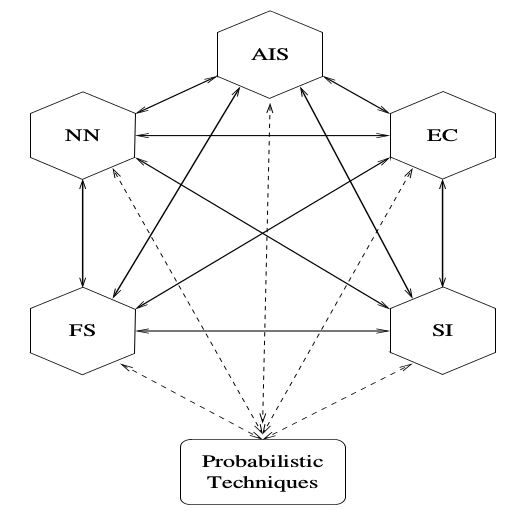
\includegraphics[scale=0.35]{../resources/paradigmas-inteligencia-computacional}
	\caption{Los algoritmos inteligentes o paradigmas de la inteligencia computacional}
	\label{fig:paradigmas-inteligencia-computacional}
\end{figure}
Mientras que las distintas técnicas de estos paradigmas han sido aplicados de forma exitosa para solucionar problemas del mundo real, la tendencia actual consiste en desarrollar hibridaciones de estos paradigmas debido a que ninguno es superior a los demás en todos los escenarios.
De esta forma, se permite rescatar y enfocarse en las fortalezas de los componentes de un sistema híbrido, eliminando sus debilidades.

Cada uno de los paradigmas previamente mencionados ha tenido su origen en sistemas biológicos.
Las redes neuronales modelan sistemas neurológicos presentes en los seres vivos, el cómputo evolutivo modela la evolución natural (incluyendo evolución genética y de comportamiento), la inteligencia de enjambre modela el comportamiento social de organismos viviendo en enjambres o colonias, los sistemas inmunes artificiales modelan el sistema inmune humano, y lós sistemas difusos se originaron a partir de los estudios de cómo los organismos interactúan con su entorno.

\section{Introducción a la inteligencia de enjambre}
Supongamos que un grupo de amigos busca un tesoro y conocen aproximadamente dónde se encuentra.
Los integrantes del grupo acuerdan un mecanismo para compartir el tesoro de modo que todos los que participan sean recompensados, pero la persona que lo encuentra tenga una recompensa mayor y que el resto de los integrantes reciba una recompensa proporcional a la distancia a la que se encontraban cuando el tesoro fue descubierto.
Supóngase además que cada integrante tiene un detector de metal y puede comunicar la intensidad de la señal y su ubicación a sus vecinos más cercanos.
De esta forma, cada persona sabe si alguno de sus vecinos está más cerca del tesoro que ella misma.
Al saberlo, se pueden tomar dos acciones:
\begin{itemize}
	\item Ignorar a los amigos, si una persona lo encuentra será por completo para ella, pero si no lo encuentra se queda con las manos vacías.
	\item Utilizar la información de los vecinos y moverse en la dirección del amigo más cercano con la señal más intensa (el que está más cerca del tesoro).
	Al utilizar la información local, se incrementan las posibilidades de encontrar el tesoro, o al menos de maximizar la recompensa.
\end{itemize}

El anterior es un ejemplo extremadamente simple de los beneficios de la cooperación en situaciones donde un sólo integrante no tiene el conocimiento total o global del entorno.
Los individuos del grupo interactúan entonces para solucionar el objetivo global al intercambiar información disponible localmente, lo cual al final se propaga a todo el grupo de tal forma que el problema se resuelve de forma más eficiente que lo que podría realizar un individuo.
En términos muy amplios, el grupo puede ser considerado un \textbf{enjambre}.
Formalmente, un enjambre puede ser definido como u\emph{n grupo de agentes (generalmente móviles) que se comunican entre ellos para actuar en su entorno local}.
Las interacciones entre agentes resultan en estrategias colectivas de solución de problemas distribuídas.

La inteligencia de enjambre se refiere al comportamiento que permite solucionar problemas y que emerge de la interacción entre dichos agentes, y la inteligencia computacional de enjambre se refiere a modelar algorítmicamente este comportamiento.
Formalmente, la inteligencia de enjambre \emph{es la propiedad de un sistema que permite que a partir del comportamiento colectivo de agentes simples que interactúan localmente con su entorno, emerjan patrones globales de funcionamiento coherente}.
La inteligencia de enjambre ha sido también denominada como \emph{inteligencia colectiva}.


\section{Optimización por cúmulo de partículas}

La inteligencia de enjambre se originó del estudio de colonias o enjambres de organismos sociales.
Los estudios del comportamiento social de organismos o individuos en cúmulos propició el diseño de algoritmos de clustering y optimización muy eficientes.
Por ejemplo, estudios de la simulación de la impredecible coreografía del vuelo de aves permitió el diseño del algoritmo de optimización por cúmulo de partículas (PSO), mientras que el estudio del comportamiento de las hormigas resultó en los algoritmos de optimización de colonia de hormigas.


PSO es un enfoque de optimización estocástico basado en el comportamiento social del vuelo de bandadas de aves.
PSO es un procedimiento de búsqueda basado en poblaciones en el que los individuos, llamados \textbf{partículas}, son agrupados en un cúmulo - nube - enjambre.
Cada partícula en el enjambre representa una solución candidata al problema de optimización.
En un sistema PSO, cada partícula \emph{vuela} a través del espacio de búsqueda multidimencional, ajustando su posición en el espacio de acuerdo a su propia experiencia y a la de las partículas vecinas.
Por lo tanto, una partícula hace uso de la mejor posición encontrada por ella misma y de la mejor posición encontrada por sus vecinos para dirigirse hacia una solución óptima.
El efecto es que las partículas vuelan hacia un óptimo, al mismo tiempo que se mantienen en búsqueda dentro de una área amplia alrededor de la mejor solución actual.
El desempeño de cada partícula (su cercanía hacia el mínimo global) es medido de acuerdo a una función de aptitud predefinida que está relacionada al problema que se intenta solucionar.
Las aplicaciones del PSO incluyen funciones de aproximación, clústering, optimización de estructuras mecánicas, así como solución de sistemas de ecuaciones.

El estudio de colonias de hormigas ha contribuido en abundancia al conjunto de algoritmos inteligentes.
El modelado del depósito de feromonas realizado por las hormigas en su úsqueda por la ruta más corta hacia los alimentos resultó en el desarrollo de los algoritmos de optimización de la ruta más corta.
Otras aplicaiones de la optimización por colonia de hormigas incluyen la optimización del ruteo en redes de telecomunicaciones, coloreado de grafos, calendarización y la colución del problema de asignación cuadrático.
Estudios de la estrucutura de los nidos de abejas y hormigas ha permitido el desarrollo de algoritmos de optimización de estructuras y clustering.




\subsection{Algoritmo PSO básico}
Los individuos en un enjambre de partículas siguen un comportamiento muy simple: emular el éxito de los individuos veicinos.
El comportamiento colectivo que emerge de este comportamiento individual es el de descubrir regiones óptimas en un espacio de búsqueda de alta dimensionalidad.
Un algoritmo PSO mantiene una lista de partículas, donde cada una de ellas representa una solución potencial.
Haciendo una analogía con el paradigma de computación evolutica, un enjabre es similar a una población, mientras que una partícula es similar a un individuo.
En términos simples, las partículas vuelan hacia un espacio de búsqueda multidimensional, donde la posición de cada partícula es ajustada de acuerdo a su propia experiencia y a la de sus vecinos.


Sea $\mathbf{x}_i(t)$ que denota la posición de la partícula $i$ en el espacio de búsqueda en el instante de tiempo $t$ (normalmente pasos de tiempo discretos).
La posición de la partícula es modificada al añadir una velocidad, $\mathbf{v}_i(t)$, a la posición actual, como:
\begin{equation}
	\mathbf{x}_i(t+1) = \mathbf{x}_i + \mathbf{v}_i(t+1)
	\label{eq:velocidad-particula-generica}
\end{equation}
con $\mathbf{x}_i(0) \sim U(\mathbf{x}_\text{min},\mathbf{x}_\text{max}$).
Es este vector de velocidad el que dirige al proceso de optimización y refleja tanto el conocimiento empírico de la partícula como la información obtenida del vecindario de la partícula.
Cada partícula recuerda las coordenadas de la mejor solución (fitness) encontrada en el espacio del problema. 
Este valor es conocido como \emph{pbest} (personal best) y representa el componente cognitivo que la partícula ha obtenido de forme empírica.
Otro \emph{mejor} valor que se almacena es el \emph{gbest} (global) que se refiere a la mejor solución, y su ubicación, obtenida por cualquier partícula del enjambre.
Originalmente, dos algoritmos PSO han sido desarrollados \emph{gbest} (global) y \emph{lbest} (local), siendo su única diferencia el tamaño de sus vecindarios.
En otras palabras, los algoritmos difieren en la forma en que calculan la velocidad de la partícula, que a su vez es utilizada para calcular la posición de la partícula según la Ecuación~\ref{eq:velocidad-particula-generica}.
El concepto básico del PSO consite en, a cada instante de tiempo, cambiar la velocidad (acelerar) cada partícula hacia su \emph{pbest} y \emph{gbest} (en la versión global).
Estas aceleraciones son ponderadas por un elemento aleatorio.


\subsubsection{Algoritmo PSO mejor global (\emph{gbest})}
Para el algoritmo PSO global best, el vecindario de cada partícula es el enjambre completo, lo cual se refleja en la topología de red.
Esto quiere decir que bajo esta topología, el componente social para actualizar la velocidad de la partícula se basa en la mejor posición encontrada en todo el enjambre, denominada $\mathbf{\hat{y}}(t)$.

En el PSO \emph{gbest}, la velocidad de la partícula $i$ es calculada como:
\begin{equation}
	v_{ij}(t+1) = v_{ij}(t) + c_1r_{1j}(t)[y_{ij}(t) - x_{ij}(t)] + c_2 r_{2j}(t)[\hat{y}_j(t) - x_{ij}(t)]
	\label{eq:velocidad-gbest}
\end{equation}
	
donde $v_{ij}(t)$ es la velocidad de la partícula $i$ en la dimensión $j$ en el tiempo $t$, $x_{ij}(t)$ es la posición de la partícula $i$ en la dimensión $j$, en el tiempo $t$, $c_1$ y $c_2$ son constantes de aceleración positiva utilizadas para escalar la contribución de los componentes cognitivos y sociales, respectivamente.
$r_{1j}(t), r_{2j}(t) \sim U(0,1)$ son valores aleatorios en el rango [0,1] muestrados con una distribución uniforme.
Estos valores aleatorios introducen un elemento estocástico al algoritmo.

La mejor posición personal, $\mathbf{y}_i$ asociada con la partícula $i$ es la mejor posición que la partícula ha visitado desde el tiempo $t(0)$.
Considerando problemas de minimización, la mejor posición en el tiempo $t+1$ se calcula como:
\begin{equation}
\mathbf{y}_i(t+1) = \begin{cases}
               \mathbf{y}_i(t)	& \text{if } f(\mathbf{x}_i(t+1)) \geq f(\mathbf{y}_i(t))\\
               \mathbf{x}_i(t+1)	& \text{if } f(\mathbf{x}_i(t+1)) < f(\mathbf{y}_i(t))\\
           \end{cases}	
\end{equation}
donde $f: \mathbb{R}^{n_x} \to \mathbb{R}$ es la función de aptitud.

La mejor posición global, $\mathbf{\hat{y}}(t)$, en el tiempo $t$ se define como:
$$
\mathbf{\hat{y}}(t) \in \left \{ \mathbf{y}_0(t), \ldots, \mathbf{y}_{n_s}(t) \right \} | | f(\mathbf{\hat{y}}(t)) = \text{min} \left \{ f(\mathbf{y}_0(t)),\ldots,f(\mathbf{y}_{n_s}(t)) \right \}
$$
donde $n_s$ es el número total de partículas en el enjambre.

El algoritmo PSO \emph{gbest} se muestra en el Algoritmo~\ref{alg:algoritmo-pso-gbest}.

\begin{algorithm} 
\begin{algorithmic}[1] 
\STATE Crear e inicializar un enjambre de $n_x$ dimensiones
\REPEAT
	\FOR {cada partícula i = 1, $\ldots$, $n_s$}
		\STATE // Establecer la mejor posición personal
		\IF { $f(x_i) < f(y_i)$ }
			\STATE $y_i = x_i$
		\ENDIF
		\STATE // Establecer la mejor posición global 
		\IF {$f(y_i) < f(\hat{y})$}
			\STATE $\hat{y} = y_i$
		\ENDIF
	\ENDFOR
	\FOR {cada partícula i = 1, $\ldots$, $n_s$}
		\STATE Actualizar la velocidad utilizando \ref{eq:velocidad-gbest}
		\STATE Actualizar la posición utilizando la ecuación \ref{eq:velocidad-particula-generica}
	\ENDFOR
\UNTIL {se cumpla la condición de paro}
\end{algorithmic} 
\caption{Algoritmo PSO \emph{gbest}} 
\label{alg:algoritmo-pso-gbest}
\end{algorithm}

El comportamiento de las partículas con este algoritmo es ejemplificado en la Figura~\ref{fig:gbest-behavior}.
\begin{figure}[]
	\centering
	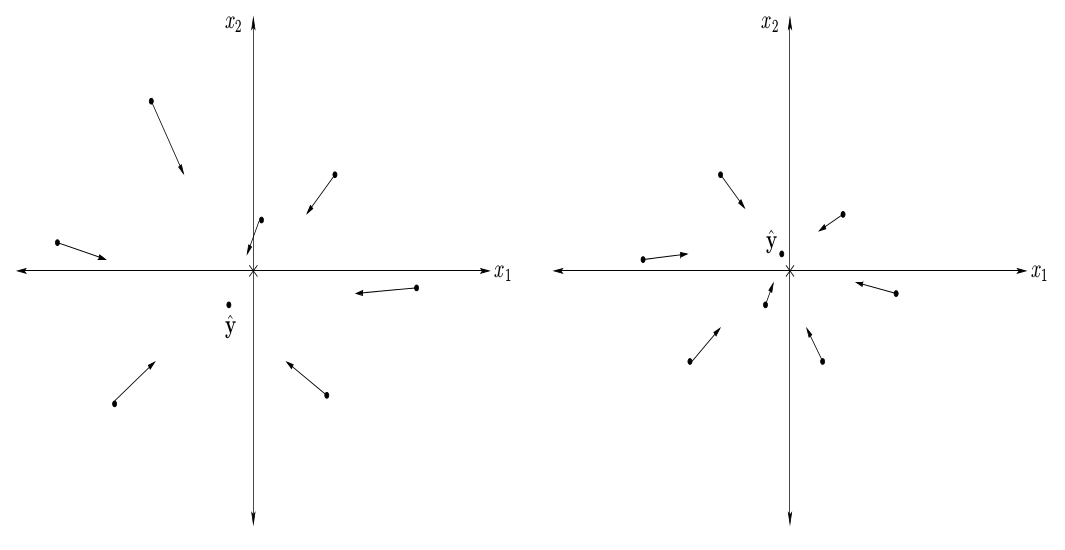
\includegraphics[width=\textwidth]{../resources/gbest-behavior}
	\caption{Comportamiento de las partículas en algoritmo gbest, $t_0$ y $t_1$}
	\label{fig:gbest-behavior}
\end{figure}
\subsubsection{Algoritmo PSO mejor local (\emph{lbest})} 
El algoritmo \emph{local best} utiliza una topología de anillo donde se definen vecindarios pequeños para cada partícula, por lo que el conocimiento del entorno es local.
En referencia a la ecuación de la velocidad, la contribución de este conocimiento local a la velocidad de la particula es proporcional respecto a la distancia que existe entre la partícula y la mejor posición encontrada por las partículas vecinas.
La velocidad se calcula como:
\begin{equation}
	v_{ij}(t+1)=v_{ij}(t) + c_1 r_{1j}[y_{ij}(t) - x_{ij}(t)] + c_2 r_{2j}(t) [\hat{y}_{ij}(t) - x_{ij}(t)]
	\label{eq:velocidad-lbest}
\end{equation}
donde $\hat{y}_{ij}$ es la mejor posición encontrada por el vecindario de la partícula $i$ en la dimensión $j$.
La mejor posición local de la partícula, $\mathbf{\hat{y}}_i$ es la mejor posición encontrada en el vecindario $\mathcal{N}_i$ y se define como:
$$
\mathbf{\hat{y}}_i (t+1) \in \left \{ \mathcal{N}_i | f( \mathbf{\hat{y}}_i (t+1) ) = \text{min} \left \{ f(x) \right \}, \forall \mathbf{x} \in \mathcal{N}_i \right \}
$$

Mientras que el vecindario se define como:
$$
\mathcal{N}_i = \left \{ y_{{i-n}_{\mathcal{N}_i}}(t), y_{i-n_{\mathcal{N}_i}+1 }(t), \ldots, y_{i-1}(t), y_{i+1}(t), \ldots, y_{i+n_{\mathcal{N}_i} }(t) \right \}
$$

Es importante noar que las partículas dentro de un vecindario no tienen relación entre ellas.
La selección de los vecindarios normalmente se realiza en base a los índices de las partículas, siendo esta tipo de selección la preferida por dos razones principales:
\begin{itemize}
	\item Es computacionalmente \emph{barato}, dado que ordenar las partículas no es requerido. 
	Algunos enfoques requieren calcular la distancia entre las partículas, por lo que la distancia euclidianada entre todos los pares de partículas debe ser calculado, lo cual es de complejidad $\mathcal{O}(n_s^2)$
	\item Ayuda a promover la distribución de la información al relacionar buenas soluciones a todas las partículas, sin importar su distribución en el espacio de búsqueda.
\end{itemize}
Es importante notar que los vecindarios se traslapan.
Dicha interconexión permite la compartición de información entre vecindarios, asegurando que el enjambre converge en un solo punto, llamado la mejor partícula global.
El algoritmo PSO \emph{gbest} es un caso especial del \emph{lbest} con $n_{\mathcal{N}_i} = n_s$

El algoritmo \emph{lbest} se desarrolla en Algoritmo~\ref{alg:algoritmo-pso-lbest}
\begin{algorithm} 
\begin{algorithmic}[1] 
\STATE Crear e inicializar un enjambre de $n_x$ dimensiones
\REPEAT
	\FOR {cada partícula i = 1, $\ldots$, $n_s$}
		\STATE // Establecer la mejor posición personal
		\IF { $f(x_i) < f(y_i)$ }
			\STATE $y_i = x_i$
		\ENDIF
		\STATE // Establecer la mejor posición global 
		\IF {$f(y_i) < f(\hat{y})$}
			\STATE $\hat{y} = y_i$
		\ENDIF
	\ENDFOR
	\FOR {cada partícula i = 1, $\ldots$, $n_s$}
		\STATE Actualizar la velocidad utilizando \ref{eq:velocidad-lbest}
		\STATE Actualizar la posición utilizando la ecuación \ref{eq:velocidad-particula-generica}
	\ENDFOR
\UNTIL {se cumpla la condición de paro}
\end{algorithmic} 
\caption{Algoritmo PSO \emph{lbest}} 
\label{alg:algoritmo-pso-lbest}
\end{algorithm}

El comportamiento de las partículas en este algoritmo es ejemplificado en la Figura~\ref{fig:lbest-behavior}.
\begin{figure}[]
	\centering
	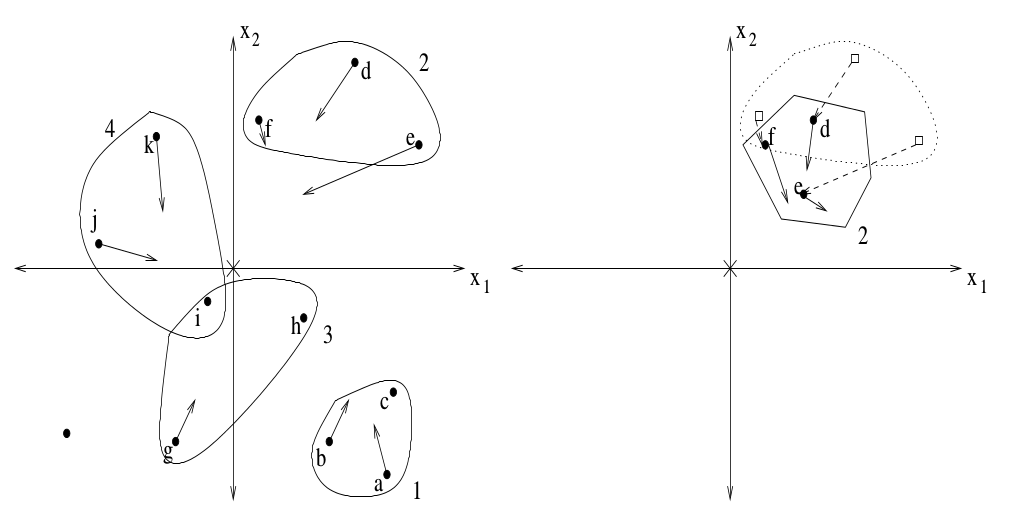
\includegraphics[width=\textwidth]{../resources/lbest-behavior}
	\caption{Comportamiento del algoritmo lbest, obsérvese al cluster 2}
	\label{fig:lbest-behavior}
\end{figure}

Al comparar las versiones \emph{lbest} y \emph{gbest} se observa que:
\begin{itemize}
	\item Debido a la mayor interconectividad de partículas, el PSO \emph{gbest} converge más rápido.
	Sin embargo, esto viene con el costo asociado de menor diversidad que el PSO \emph{lbest}.
	\item Como consecuencia de la mayor diversidad alcanzada por \emph{lbest} (lo cual resulta en porciones más grandes del espacio de búsqueda cubiertas), el PSO \emph{lbest} es menos suceptible a mínimos locales.
	En general, las estructuras de vecindarios como la topología anillo utilizada en PSO \emph{lbest} ofrecen el mejor desempeño.
\end{itemize}


\subsubsection{Parámetros del PSO}
\begin{itemize}
	\item \textbf{Tamaño del enjambre, $n_s$}: a mayor cantidad de partículas habrá mayor diversidad inicial en el enjambre y se podría cubrir un mayor espacio de soluciones.
	Adicionalmente, una gran cantidad de partículas podría acelerar la convergencia, aunque aumentaría la complejidad.
	\item \textbf{Tamaño del vecindario}: mientras más pequeño sea el tamaño de los vecinos habrá menor interacción, la convergencia será más lenta, pero será más fácil converger en soluciones óptimas.
	Es posible iniciar con vecindarios pequeños y luego incrementar su tamaño sobre la marcha.
	\item \textbf{Número de iteraciones}: depende del escenario, pocas iteraciones podrían terminar la búsqueda prematuramente; muchas iteraciones podrían provocar la ejecución de iteraciones innecesarias.
	\item \textbf{Coeficientes de aceleración}, $c_1$ y $c_2$: controlan la influencia estocástica de los componentes personales (o locales) y sociales sobre la velocidad general de una partícula. $c_1$ indica la \emph{confianza} de una partícula en sí misma, y $c_2$ la confianza que tiene en el vecindario.
\end{itemize}

\subsubsection{Condiciones de paro} 
Las siguientes son las condiciones de paro más comunes:
\begin{itemize}
	\item Un número máximo de iteraciones.
	\item Una solución aceptable es encontrada: $f(x_i) \leq |f(x^*) - \epsilon |$
	\item No existe una mejora después de un número de iteraciones.
	\item El radio del enjambre normalizado es cercano a 0.
	\item Terminar cuando la pendiente de la función objetivo es aproximadamente 0.
\end{itemize}

\subsection{Variantes de PSO}
El PSO básico ha sido utilizado exitosamente a gran cantidad de problemas como problemas estándar de optimización de funciones, permutaciones y entrenamiento de redes neuronales de múltiples capas.
Sin embargo, su aplicación también ha permitido identificar deficiencias para converger a buenas soluciones.
Varias modificaciones básicas al PSO han sido desarrolladas para mejorar la rapidez y calidad de soluciones.
Estas modificaciones incluyen la introducción de un peso de inercia, \emph{sujeción} (clamping) de velocidad, \emph{estrechamiento} (constriction) de velocidad, así como distintos mecanismos para determinar los mejores personales y globales (o locales), así como los diferentes modelos de velocidad.

\paragraph{Sujeción de velocidad}
El compromiso exploración - explotación es un aspecto importante que determina la eficiencia y precisión de un algoritmo de optimización.
Exploración es la habilidad para explorar diferentes regiones del espacio de búsqueda para encontrar un valor óptimo.
Explotación es la habilidad para concentrar la búsqueda alrededor de un área prometedora.
Dichos objetivos son tratados por la ecuación de actualización de velocidad.
La sujeción o restricción de velocidad limita la velocidad de las partículas para permanecer dentro de un umbral.
Si una partícula excede a dicha velocidad, es entonces acotada en este valor $V_{\text{max}}$.
Usualmente, $V_{\text{max}}$ en la dimensión $j$ se establece como una fracción del dominio de dicha dimensión.
Este acotamiento se realiza justo después de calcular la nueva velocidad en el algoritmo.

\paragraph{Peso de inercia}
El peso de inercia es un mecanismo que intenta suplir al parámetro de sujeción de velocidad.
El peso de inercia $\omega$ controla el \emph{momentum} de la partícula al ponderar la contribución de la velocidad anterior.
En otras palabras, controla qué tanta memoria de la dirección del vuelo anterior infuirá en la nueva velocidad.
Entonces, la ecuación de velocidad cambia a:
\begin{equation}
	v_{ij}(t+1) = \omega v_{ij}(t) + c_1r_{1j}(t)[y_{ij}(t) - x_{ij}(t)] + c_2 r_{2j}(t)[\hat{y}_j(t) - x_{ij}(t)]
	\label{eq:velocidad-peso-inercia}
\end{equation}

Existen varios enfoques para cambiar este peso, ajustes aleatorios, decremento lineal y no-lineal, adaptación difusa y ajuste incremental.

\paragraph{Coeficiente de estrechamiento de velocidad}
Es un mecanismo similar al peso de inercia para balancear el compromiso exploración - explotación.
La ecuación de actualización de la velocidad cambia a:
\begin{equation}
	v_{ij}(t+1) = \mathcal{X} [ v_{ij}(t) + \phi_1 (y_{ij}(t) - x_{ij}(t)) + \phi_2(\hat{y}_j(t) - x_{ij(t)})   ]
\end{equation}
donde
$$
\mathcal{X} = \frac{2 \kappa}{| 2 - \phi - \sqrt{\phi ( \phi - 4)}  |}
$$
y $\phi = \phi_1 + \phi_2$, $\phi_1 = c_1 r_1$ y $\phi_2 = c_2 r_2$.
Debería mantenerse que  $\phi \geq 4$ y $\kappa \in [0,1]$, según se ha derivado de un análisis formal de eigenvalues de la dinámica de enjambres.


\paragraph{Actualizaciones síncronas o asíncronas de las mejores posiciones}
Las versiones iniciales de PSO realizan la actualización de las mejores posiciones de forma aislada respecto a las actualizaciones de las posiciones de las partículas.
Es posible realizar la actualización de las mejores posiciones después de la actualización de cada partícula, mejorando el desempeño de \emph{lbest}.

\paragraph{Modelos de velocidad}
Existen modelos alternativos que difieren en los componentes incluidos en la ecuación de la velocidad y cómo las mejores posiciones son calculadas.
\begin{itemize}
	\item \textbf{El enfoque solamente individual (cognition-only model)} excluye al componente social de la ecuación de la velocidad.
	Esto puede recordar a la \emph{nostalgia} en el sentido de que existe una tendencia estocástica de que las partículas retornen hacia su anterior mejor posición.
	\item \textbf{El enfoque solamente social} excluye el componente individual de la ecuación de la velocidad.
	Todas las partículas son atraídas hacia la mejor posición de su vecindario.
	\item \textbf{El enfoque desinteresado (selfless mode)} es básicamente el modelo social, pero la mejor solución del vecindario se obtiene de una partícula vecina.
	En otras palabras, no se le permite a la partícula por sí misma convertirse en la mejor del vecindario.
\end{itemize}

\subsection{Vecindarios y topologías}
La característica que dirige al PSO es la interacción social.
En este sentido, la estructura social del PSO se determina por la formación de los vecindarios con traslape, en la que las partículas de un vecindario influyen en otro vecindario.
Por ello, el desempeño del PSO depende ampliamente en la estructura de la red social.
Más específicamente, el flujo de información a través de una red social depende de:
\begin{itemize}
	\item El grado de conectividad entre los miembros de la red,
	\item La cantidad de agrupamiento (los vecinos de un nodo son también vecinos de otro)
	\item La distancia promedio más corta de un nodo a otro.
\end{itemize}

En una red altamente conectada, hay mayor comunicación entre los individuos y se converge más rápido, sin embargo se es más susceptible a los óptimos locales debido a que se cubre un menor espacio de búsqueda.
Las siguients son las topologías más comunes para las redes establecidas en PSO:
\begin{itemize}
	\item \textbf{Estrella}: Cada partícula se interconecta con cada una de las demás.
	La primera implementación de PSO utilizó esta topología.
	PSO \emph{gbest} converge más rápido pero es susceptible a óptimos locales.
	\item \textbf{Anillo}: Cada partícula se comunica con sus $n_\mathcal{N}$ vecinos inmediatos.
	Es utilizado por \emph{lbest}. Converge en un tiempo mayor pero ofrece una mayor cobertura del espacio de búsqueda.
	\item \textbf{Rueda}: Las partículas de un vecindario se aislan de las otras.
	Una partícula funciona como partícula foco, la cual compara el desempeño de las partículas de su vecindario y ajusta su posición hacia la del mejor; si la posición de la partícula foco es mejor que la de sus vecinas, propaga su posición hacia ellas.
	\emph{Enlentece} la propagación de las buenas soluciones hacia el enjambre.
	\item \textbf{Pirámide}: Forma un \emph{wire-frame} tridimensional.
	\item \textbf{Cuatro clústers}: En esta estructura, cuatro clústers se forman con dos conexiones entre ellos.
	Las partículas dentro de cada clúster se conectan con cinco vecinos.
	\item \textbf{Von Neumann}: Las partículas se conectan en un grid.
\end{itemize}



\nocite{*}
\bibliographystyle{plain}
\bibliography{../resources/references} 

\end{document}